\documentclass[letterpaper,twocolumn,openany,nodeprecatedcode]{dndbook}

% Use babel or polyglossia to automatically redefine macros for terms
% Armor Class, Level, etc...
% Default output is in English; captions are located in lib/dndstring-captions.sty.
% If no captions exist for a language, English will be used.
%1. To load a language with babel:
%	\usepackage[<lang>]{babel}
%2. To load a language with polyglossia:
%	\usepackage{polyglossia}
%	\setdefaultlanguage{<lang>}
% \usepackage[english]{babel}
%\usepackage[italian]{babel}
% For further options (multilanguage documents, hypenations, language environments...)
% please refer to babel/polyglossia's documentation.

\usepackage[german]{babel}
\usepackage[singlelinecheck=false]{caption}
\usepackage{lipsum}
\usepackage{listings}
\usepackage{shortvrb}
\usepackage{stfloats}
\usepackage{tikz}
\setcounter{chapter}{-1}

\captionsetup[table]{labelformat=empty,font={sf,sc,bf,},skip=0pt}

\MakeShortVerb{|}

\lstset{%
  basicstyle=\ttfamily,
  language=[LaTeX]{TeX},
  breaklines=true,
}

\title{Der magische Wald von Aestheros \\
\large Ebene Avis}
\author{Max Schmitt}
\date{\today}

\begin{document}

\frontmatter
\maketitle
\tableofcontents
\mainmatter

\chapter{Die Weltenebene Avis}

\DndDropCapLine{D}{ie Göttin Vehnera,} letzte Tochter der Urgöttin Argdea und dem Urgott der Zeit Rhaneires, war all das Elend auf den Welten-Ebenen der anderen Götter leid. Sie empfand es als schrecklich, die ganze Zeit zusehen zu müssen, wie die anderen Götter sich an den Schmerzen und der Schreie der ganzen Wesen ergötzten.

 All jenes Leid, den Tod, den Schmerz. Dies wollte Vehnera nicht. So beschloss sie nun eine Welt ohne all diese Probleme zu erschaffen. Sie war der festen Überzeugung, dass die Hauptursache der Indikator Magie war, den die anderen Götter zu ihrer belustigung mit in die Welt gaben. Der Gedanke von einer Welt ganz ohne Magie war bis zu diesem Zeitpunkt neu. So bekam sie von ihrer Mutter der Urgöttin Argdea unterstützung.

Sothos, ihr Bruder der ihr bis dahin am nächsten Stand, lehnte sich jedoch aus Neid um die Gunst der Mutter dagegen auf und wurde zur Strafe für ein Jahrhundert nach Avis verbannt. Er sollte sehen, dass die Wesen, erschaffenen nach dem Abbild der anderen Ebenen, es besser haben ohne Magie. Sothos jedoch sah und verstand, dass das Problem nicht an der Magie liegen konnte und die Menschen sogar mehr litten. Auch er litt eine lange Zeit als unsterblicher Humanoider auf der Welt und kehrte mit großem Mitleid zurück auf die Ebene der Götter.

Enttäuscht und getrieben von der neuen Emotion Wut die er bei den Humanoiden lernte, lehnte er sich gegen Argdea und Vehnera auf. Rhaneires, sein Vater und Urgott der Materie beschloss, dass Sothos eine Teilmacht an Avis bekommen sollte, wenn er denn aufhörte sich aufzulehnen. So beschlossen Vehnera und Sothos sich Avis zu teilen. Sie waren sich einig, dass es sich schon herauskristalisieren würde, wer denn die glücklichere Wesen hätte. So schenkte Sothos halb Avis magische Kräfte.

\textit{Dieses Abenteuer spielt nach einer Zeit der Kriege, in denen viele Magier verfolgt und getötet wurden. Es herrscht im verborgenen ein Krieg der Religionen und der Götter. Nichtmagier bekämpfen Magier und auch umgekehrt.}

\section{Die Götter}
\subsection{Argdea - URGÖTTIN DER ZEIT}
Argdea, die Urgöttin, existierte beiseite der Unendlichkeit. Zusammen mit der Zeit, erschuf sie Rhaneires und gab ihm einen freien Willen um weitere Götter erschaffen und vorallem mit jemandem die einsame Zeit in der Unendlichkeit zu teilen. Argdea war getrieben auf der Suche nach Vollendung. Humanoiden würden es die wahre Liebe bezeichnen.

\subsection{Rhaneires - URGOTT DER MATERIE}
Nachdem Argdea den Urgott Rhaneires erschuf, umgarnte sie ihn mit dem Ziel neue Götter zu erschaffen. Rhaneires jedoch, erschaffen mit freiem Willen, stimmte erst ein, nachdem Argdea einwilligte ihn sein Werk vollenden zu lassen. Es war die Materie. Rhaneires wollte etwas Formbares Reines und neues erschaffen. Etwas, von dem er und jeder Gott besitz ergreifen könnte. Etwas, was er selbständig lassen und nach belieben erschaffen konnte.

\subsection{Vehnera - MUTTER DES LEBENS}
Vehnera, eine der Töchter der Urgötter, erschuf das Leben, die Natur und die Liebe auf Avis.
\begin{DndSidebar}{Vehnera, vor erschaffung von Avis}
  So viel Leid. So viel Hass. Die Waffe Magie ist der Grund. Und ihr? Ihr ergötzt euch nur an dem Leidern der Menschen! \newline
  ~ ~ \textit{Vehnera, Mutter des Lebens}
\end{DndSidebar}


\subsection{Sothos - DER VERSTOẞENE}
Nach dem Streit sah Sotos sich in der Aufgabe den Streit, Kampf, Leid und Tod der Humanoiden gerecht aufzuteilen. Im Ausgleich für ihr Leiden gab er ihnen die Magie.
\begin{DndSidebar}{Sothos auf Avis, knieend an den Sänften-Klippen auf Nesloney}
  Der Mensch, der Zwerg, der Elf. Und Alles andere was du erschufest, litt und leidet! Auch ohne Magie und noch viel mehr!  Heuchler bist du, seid ihr! Ihr alle! Alle nur Heuchler! \newline
  ~ ~ \textit{Sothos, der Verstoßene}
\end{DndSidebar}

\subsection{Organisationen und Religionen}


\subsubsection{Vehnerismus}

Normale bevölkerung

\subsubsection{Sothoismus}

Magier oder Familien von Magiern, liberale menschen "Böse geächtet"

\subsubsection{Rhaneirismus}

Es gibt einen Klan der behauptet nur Rhaneires wäre der einzig ware Gott. Sie streiten die anderen Götter nicht ab, jedoch sind sie der Meinung, dass ihr Gott ihnen die roheste nagische Kraft verleiht.
-> Machos
-> Frauenfeindlich (Frau gehört in die küche)

\subsubsection{Athenesis}
Es gibt einen nicht erkundeten Gott, der Gott der unendlichkeit. und erforschen nach weiteren urgötter
Sehr Wissenschafltich
"Unendlichkeit ist unendlich, es muss auch eine unendliche anzahl an GÖtter geben" ~ Philisoph und Gründer der Athenesis

\newpage

%\chapter{Ankunft in Aestheros}

%\includegraphics[width=\linewidth]{}
\tikz[remember picture,overlay] \node[opacity=0.8,inner sep=0pt] at (current page.center){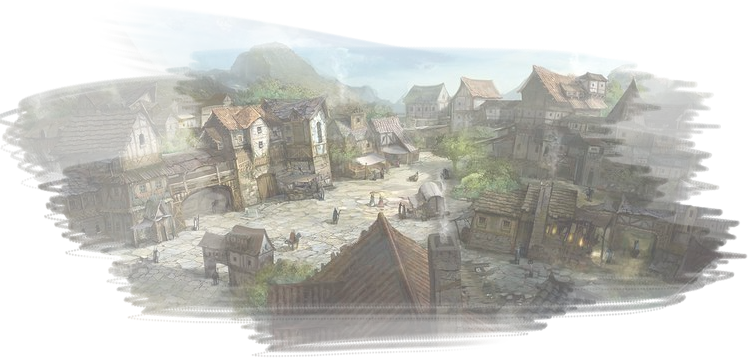
\includegraphics[width=\paperwidth]{img/world/Aestheros.png}};

\DndDropCapLine{I}{n diesem Kapitel gelangen} unsere Abenteurer das erste Mal in Kontakt mit dem Questgeber. Dem Yarl von Aestheros.

%\begin{DndReadAloud}
% \DndDropCapLine{U}{unsere %Abenteurer,}
%\end{DndReadAloud}
Die Kampagne
\begin{DndReadAloud}
Vor
\end{DndReadAloud}


Aestheros ist ein kleines Dorf auf der Ebene Avis.
.

.

Mollige Gasthausdame, überfürsorglich. Dorf-Barde, kann nicht sonderlich gut singen.

Yarl Sohn hat erkrankten Sohn. Er hat nur eine Woche laut dem Yarl-Hexer. Bietet Abenteurer GEld
Am Waldesrand steht eine Hütte. Dort wohnt ein Alter Mann. (Er wird gerade überfallen) Dieser Mann gibt ihnen eine optionen.
Hat angst, weiß nicht ob man einem trauen kann. man soll einen freund aus einer höhle retten zum beweis

Zauberin Triss aufsuchen und ein uraltes magisches Wesen. Einhorn.
Dieses Einhorn muss überzeugt werden, dass es den Sohn heilt.

Geliebte A von X zerfleischt am Waldesrand gefunden. -> Y hat X
Y verschwindet immer bei der Vollmond Nacht vor sonnenuntergang. Gerüchte -> er hat eine andere. (dabei wird er nur zu einem werwolf)

weitere Hütte -> Todkranke und ältere dame -> Heiltrank muss gebraut werden.

Verfolgen von einem unschuldigen Magier


\end{document}
